\documentclass[]{article}

%opening
\title{Mathematical modeling of hydrogen diffusion in biphasic steel.}
\author{Danilo de Freitas Naiff}

\usepackage[english]{babel}
\usepackage[utf8]{inputenc}
\usepackage[T1]{fontenc}
\usepackage{hyperref}
% \usepackage{booktabs}
\usepackage{physics}
\usepackage{siunitx}
\usepackage[version=4]{mhchem}
\usepackage{graphicx}
\usepackage{indentfirst}
\usepackage{caption}
\usepackage{tikz}
\usepackage{amsthm}
\usepackage{amssymb}
\usepackage{amsmath}
\usepackage{textcomp}
\usepackage{gensymb}
\usepackage{nomencl}
\usepackage{multirow}
\usepackage{algpseudocode}
\usepackage{subfig}
\usepackage{listings}
\usepackage{tikz}
\algnewcommand{\LineComment}[1]{\State \(\triangleright\) #1}
\makenomenclature

\newcommand{\red}{\textcolor{red}}
\newcommand{\pderiv}[2]{\frac{\partial #1}{\partial #2}}

\newcommand{\argmax}{\operatorname{argmax}}
\newcommand{\argmin}{\operatorname{argmin}}
\def \gu {{\bar{g}}}
\def \Ev {{\mathbb E}}
\def \Pr {{\mathbb P}}
\def \f {{\mathbf f}}
\def \u {{\mathbf u}}
\def \y {{\mathbf y}}
\def \x {{\mathbf x}}
\def \m {{\mathbf m}}
\newcommand{\Var}{\mathrm{Var}}
\newcommand{\Cov}{\mathrm{Cov}}

\definecolor{darkgreen}{rgb}{0,0.5,0}

% My own definitions of colors 
\definecolor{codegreen}{rgb}{0,0.6,0}
\definecolor{codegray}{rgb}{0.5,0.5,0.5}
\definecolor{codepurple}{rgb}{0.58,0,0.82}
\definecolor{backcolour}{rgb}{0.95,0.95,0.92}
% Definitions on how to display listings
\lstdefinestyle{mystyle}{
	backgroundcolor=\color{white},   
	commentstyle=\color{codegreen},
	keywordstyle=\color{blue},
	numberstyle=\tiny\color{codegray},
	stringstyle=\color{codepurple},
	basicstyle=\tiny,
	language=Python,
	breakatwhitespace=false,         
	breaklines=true,                 
	captionpos= top,%b                    
	keepspaces=true,                 
	numbers=left,                    
	numbersep=5pt,                  
	showspaces=false,                
	showstringspaces=false,
	showtabs=false,
	%stepnumber=3,                  
	tabsize=2
}

\lstset{style=mystyle}

\begin{document}

\maketitle

\begin{abstract}

\end{abstract}

\section{Model}
The main model consists of hydrogen diffusion two-phase system, in which there is a bulk phase, with spherical precipitates in it, disperse enough so that we can do homogenization. Moreover, consider that the precipitates have a radius of $R$, that the bulk diffusivity is $D$, the precipitate diffusivity is $\alpha$, and there is $\Gamma$ precipitates per unit volume (we can get this statistics from the volume fraction, assuming spherical particles).

We denote by $c(x, t)$ the hydrogen concentration at the bulk phase, while we denote by $n(r, t; x)$ the concentration of hydrogen in the precipitate at $x$, on radius $r$ (of the precipitate) and time $t$.
 
The interface between two phases satisfies both the continuity of chemical potential, which translates to
\begin{equation}
	\frac{c}{n} = \frac{S_c}{S_n} = \exp \left( \frac{\mu_c - \mu_n}{RT} \right) =: K,
\end{equation}
and the continuities of fluxes
\begin{equation}
	J_c = J_n = J.
\end{equation}

Now, consider an interface at $(x, t)$. From the point of view of the bulk, we can think of this interface as being a sink for the bulk concentration, at the boundary. Then, \textit{each precipitate} results in a volumetric sink of strength $4 \pi R^2 J$. Of course, then we have that the sink per unit volume becomes $4 \pi R^2 \Gamma J$. Therefore, we can consider the bulk transport as following a diffusion equation with sink
\begin{equation}
	\pderiv{c}{t}(x,t) = D \frac{\partial^2 c}{\partial x^2}(x,t) - 4 \pi R^2 \Gamma J.
\end{equation}

Now, from the point of view of the precipitate at $x$, we have that the continuity of chemical potentials makes that, at the interface \textit{from the precipitate size}, we can consider a time-varying inlet concentration dependant on $c(x,t)$. That is, at $r = R$ (and $r = -R$), we must have
\begin{equation}
	n(R, t; x) = c(x, t).
\end{equation}
As for the precipitate itself, it follows that it must obey the spherically symmetric form of the diffusion equation 
\begin{equation}
	\pderiv{n}{t}(r,t,x) = \alpha \frac{1}{r^2} \pderiv{}{r} \left( r^2 \pderiv{n}{r}(r,t,x)\right)
\end{equation}

And, of course, Fick's first law says that we can calculate the flux $J$ from the precipitate side, given by
\begin{equation}
	J = -\alpha \pderiv{n}{r}(R,t).
\end{equation}.
Therefore, we end up with the model as in the next section.

\section{Derivation of bulk equation}
Consider then

\begin{equation}\label{originalproblem}
	\begin{split}
	& \pderiv{c}{t}(x,t) = D \frac{\partial^2 c}{\partial x^2}(x,t) - 4 \pi R^2 \Gamma J; t \geq 0, 0 \leq x \leq L\\
	& \pderiv{n}{t}(r,t,x) = \alpha \frac{1}{r^2} \pderiv{}{r} \left( r^2 \pderiv{n}{r}(r,t,x)\right); \quad t \geq 0, -R \leq x \leq R \\
	& J = -\alpha \pderiv{n}{r}(R,t) \\
	& n(R,t,x) = n(-R,t,x) = K c(x,t) \\
	\end{split}
\end{equation}

First: solving $n$ differential equation. Ommiting $x$, let $m(r,t) := n(r,t) - c(t)$. Hence,
\begin{equation}\label{precipitatemproblem}
	\pderiv{m}{t}(r,t) = \alpha \mathcal{O}[m](r,t) + c'(t); \quad m(r,t) = m(-R,t) = 0,
\end{equation}
with
\begin{equation}
	\mathcal{O}(m) = \frac{1}{r^2} \pderiv{}{r} \left( r^2 \pderiv{m}{r} \right)
\end{equation}
Using separation of variables, let $m(r,t) = T(t) \varphi(r)$. Hence, we have
\begin{equation}
 T' \varphi = \alpha \mathcal{O}[\varphi] T + c'(t)
\end{equation}
We look then at the eigenvalue problem
\begin{equation}
\mathcal{O}[\varphi] = -\lambda \varphi,
\end{equation}
or
\begin{equation}
r^2 \varphi'' + 2 r \varphi' + \lambda r^2 \varphi = 0.
\end{equation}
The above equation equals to
\begin{equation}
(r \varphi)'' + \lambda (r \varphi) = 0.
\end{equation}
Considering $\varphi(R) = \varphi(-R) = 0$, for $\lambda_0 <= 0$, $\varphi(R) = 0$, and, for $\lambda > 0$,
\begin{equation}
(r \varphi) = R \sin (\sqrt{\lambda_k} r); \quad \sqrt{\lambda_k} = \frac{\pi k}{R}
\end{equation}
Hence, the eigenvalue problem is 
\begin{equation}\label{eigenvaluemproblem}
\varphi_k(r) = \pi k j_0(\pi k r/R); \quad \lambda_k = \frac{\pi^2 k^2}{R^2}; \quad k = 1, 2, ...
\end{equation}
with $j_0(x) = \sin(x)/x$ being the zeroth spherical Bessel function of the first kind (who is also the sinc function).

Getting already some things off the table, we have that $\varphi_k$ forms an base of functions, that has the orthonormality relations
\begin{equation}\label{orthonomalityrelations}
\frac{1}{R} \int_{-R}^R (r/R)^2 \varphi_k(r) \varphi_l(r) dr = \delta_{m,l}.
\end{equation} 
due to
\begin{equation}
\begin{split}
& \frac{1}{R} \int_{-R}^R (r/R)^2 \varphi_k(r) \varphi_l(r) dr = \\
& 2 \pi^2 k^2 \int_{0}^1 u^2 j_o(\varphi k u) j_0(\varphi l u) du = \\
& 2 \pi^2 k^2 \frac{\delta_{k,l}}{2} (j_1(\pi k))^2 = \\
& \delta_{k,l} \pi^2 k^2 \left(\frac{-(-1)^k}{\pi k}\right)^2 = \\
& \delta_{k,l}
\end{split},
\end{equation}
with $j_1(x)$ being the first spherical Bessel function of the first kind. Hence, for any (suitable) $f(r)$, we can decompose
\begin{equation}
\begin{split}
& f(r) = \sum_{k=1}^\infty f_k \varphi_k \\
& f_k(r) = \frac{1}{R} \int_{-R}^R (r/R)^2 f(r) \varphi_k(r) dr.
\end{split}
\end{equation}.
In particular, we use the decomposition
\begin{equation}
K c'(t) = \sum_{k=1}^\infty K c'_k(t) \varphi_k(t).
\end{equation}
We have that, using the eigenvalue problem, decomposing
\begin{equation}
m(r,t) = \sum_{k=1}^\infty \psi_k(t) \varphi_k(r),
\end{equation}
we have that 
\begin{equation}
\sum_{k=1}^{\infty} \left(\psi_k'(t) + \lambda_k \alpha \psi_t - c'_k(t) \right) \varphi(k) = 0,
\end{equation}
Hence, we have
\begin{equation}
\psi_k(t) = e^{-\alpha \lambda_k t} \left(\psi_k(0) + \int_0^t e^{\alpha \lambda k \tau} K c'_k(\tau) d \tau \right),
\end{equation}
or, assuming $\psi_k(0) = 0$ (because we will consider $n(0,t,x) = 0$ and $c(0,t) = 0$), 
\begin{equation}\label{phikdefinitions}
\begin{split}
\psi_k(t) & = K e^{-\alpha \lambda_k t} \int_0^t e^{\alpha \lambda k \tau} c'(\tau) \frac{1} R \int_{-R}^R (r/R)^2 \varphi_k(r) dr d \tau = \\
& = -2 K \frac{(-1)^k}{\pi k} e^{-\alpha \lambda_k t} \int_0^t e^{\alpha \lambda_k \tau} c'(\tau) d \tau = \\
& -2 K \frac{(-1)^k}{\pi k} \left(c(t) + e^{-\alpha \lambda_k t} c(0) - \frac{e^{-\alpha \lambda_k t}}{\lambda_k t} \int_0^t e^{\alpha \lambda_k t} c(\tau) d\tau \right).
\end{split}
\end{equation}
And, we remember that $m(r,t) = n(0,t) + c(t)$. Finally, we can then find
\begin{equation}
J = \alpha \pderiv{n}{r} (t,R) = -\alpha \sum_{k=1}^\infty \psi_k(t) \pderiv{\varphi_k}{r}(R).
\end{equation}.
But, we have that $\pderiv{\varphi_k}{r}(R) = (-1)^k \pi k/R$. Hence, we can join everything and find that
\begin{equation}
J = \frac{2}{R} \alpha K \sum_{k=1}^\infty \left(c(t) + e^{-\alpha \lambda_k t} c(0) - \frac{e^{-\alpha \lambda_k t}}{\lambda_k t} \int_0^t e^{\alpha \lambda_k t} c(\tau) d\tau \right).
\end{equation}
Therefore, our equation for $c$ becomes (showing again $x$):
\begin{equation}\label{bulkproblemform1}
\begin{split}
\pderiv{c}{t}(x,t) = & D \frac{\partial^2 c}{\partial x^2}(x,t) - \\
& 8 \pi R \Gamma \alpha K \sum_{k=1}^\infty \left(c(x,t) + e^{-\alpha \lambda_k t} c(x,0) - \frac{e^{-\alpha \lambda_k t}}{\lambda_k t} \int_0^t e^{\alpha \lambda_k t} c(x, \tau) d\tau \right),
\end{split}
\end{equation}
or
\begin{equation}\label{bulkproblemform2a}
\pderiv{c}{t}(x,t) = D \frac{\partial^2 c}{\partial x^2}(x,t) - 8 \pi R \Gamma \alpha K \sum_{k=1}^\infty e^{-\alpha \lambda_k t} \int_0^t e^{\alpha \lambda_k \tau} c'(\tau) d \tau
\end{equation}
or still
\begin{equation}\label{bulkproblemform2b}
\begin{split}
& \pderiv{c}{t}(x,t) = D \frac{\partial^2 c}{\partial x^2}(x,t) - 8 \pi R \Gamma \alpha K \sum_{k=1}^\infty (\omega_k *_t c')(x,t) \\
& \omega_k(t) = \exp \left( -\frac{\alpha \pi^2 k^2 t}{R^2} \right),
\end{split}
\end{equation}
with $(f *_t g)(x,t) = \int_0^t f(x, t - \tau) g(x, tau) d\tau $ being the convolution evaluated in the $t$ argument.

Of course, we can simplify things by making
\begin{equation}\label{auxiliarydefinitions2}
	\begin{split}
	& \beta := 8 \pi R \Gamma \alpha K \\
	& \omega := \sum_{k=1}^\infty \omega_k = \sum_{k=1}^\infty \exp \left( -\frac{\alpha \pi^2 k^2 t}{R^2} \right)
	\end{split},
\end{equation}
resulting in \eqref{bulkproblemform2b} being written as
\begin{equation}\label{bulkproblemform2}
	\pderiv{c}{t} + \beta \left(\omega *_t \pderiv{c}{s}\right) = D \frac{\partial^2 c}{\partial x^2},
\end{equation}
or, expanding the convolution,
\begin{equation}\label{bulkproblemform3}
	\pderiv{}{t} c(x, t) + \beta \int_0^t \omega(t - s) \pderiv{}{s} c(x, s) ds = D \frac{\partial^2 c}{\partial x^2}(x,t)
\end{equation}

\subsection{Cylindric precipitates, \textit{mutatis mutandis}}
If we consider the approximation by cylindric precipitates, then, defining $\Gamma_c$ as the amount precipitates per cross-sectional area, we can follow the same arguments above (now using Bessel functions of the first kind), and arrive at almost the same equations, now with
\begin{equation}
	\begin{split}
		& \beta = 4 \pi \Gamma \alpha K \\
		& \omega = \sum_{k=1}^\infty \omega_k = \sum_{k=1}^\infty \exp \left( -\frac{\alpha u_{0, k}^2 t}{R^2} \right)
	\end{split},
\end{equation}
with $u_{0, k}$ being the k-th zero of the zeroth Bessel function of the first kind.

\section{Discretization}
Let's discretize this. Forgetting about $x$ for now, consider only the operator
\begin{equation}
	\pderiv{}{t} c(t) + \beta \int_0^t \omega(t - s) \pderiv{}{s} c(s) ds.
\end{equation}
Now, consider a discretization
\begin{equation}
	\begin{split}
	& t_0, t_1, \ldots, t_n, t_{n+1} \\
	& c_0, c_1, \ldots, c_n, c_{n+1} \\
	& h_i := t_{i} - t_{i-1} \\
	& t_{i+1/2} = (t_{i+1} - t_{i})/2
	\end{split}
\end{equation}
Then, we can discretize the integral at time $t_{n+1}$ by
\begin{equation}
	\int_0^t \omega(t - s) \pderiv{}{s} c(s) ds \approx \sum_{i=0}^n \omega(t_{n+1} - t_{i+{1/2}}) (c_{i+1} - c_{i}).
\end{equation}
Separating the $c_{n+1}$ from the rest, and defining $\omega^{n+1, i}$ as $\omega(t_{n+1} - t_{i+{1/2}})$, we have the discretization as a function of $c_{n+1}$
\begin{equation}
	\frac{c_{n+1} - c_{n}}{h_{n+1}} + \beta (c_{n+1} - c_n) \omega^{n+1, n} + \beta \sum_{i=0}^{n-1} (c_{i+1} - c_i) \omega^{n+1, i},
\end{equation}
or
\begin{equation}
	\left(\frac{1}{h_{n+1}} + \beta \omega^{n+1, n} \right) c_{n+1} - \left(\frac{1}{h_{n+1}} + \beta \omega^{n+1, n} \right) c_{n} + \beta \sum_{i=0}^{n-1} (c_{i+1} - c_i) \omega^{n+1, i}.
\end{equation}

Now, considering the space discretization \footnote{can be finite differences, elements, or whatever}, let the discretized operator matrix be $A$ letting $\mathbf{c}$ be the space discretization vector, we have that, using the implicit Euler method, the above problem translates to (rewritten so that we guarantee a positive diagonal)
\begin{equation}
 \begin{split}
 & \left(-A + (h_{n+1}^{-1} + \beta \omega^{n+1, n}) I \right)\mathbf{c}_{n+1} = \\
 & -\beta \sum_{i=0}^{n-1} (\mathbf{c}_{i+1} - \mathbf{c}_i) \omega^{n+1, i} + \left(h_{n+1}^{-1} + \beta \omega^{n+1, n} \right) \mathbf{c}_{n},
 \end{split}
\end{equation}
which we can then solve at each time step. Some notes here
\begin{itemize}
	\item In practice, $\omega$ decays as $t_{n+1} - t_i$ grows large. Can probably do some cutoff here.
	\item If we use a constant time step, we can define $\hat{\omega}^j := \omega^{n+1, n-j} = \omega(h(j + 1/2))$. We just calculate beforehand for some values of $j$ and hold the values (remembering the cutoff note above).
\end{itemize}

\section{Results}
There are the results of a simulation of this model, with unit concentration at the inlet and zero concentration at the outlet.
\begin{itemize}
	\item Physical parameters (some taken from Olden)
	\begin{itemize}
		\item $D$ - 6.0*1e-1 $\mu m^2/s$
		\item $\alpha$ - 1.4*1e-4 $\mu m^2/s$
		\item $K$ - 32.51/0.033
		\item $R$ = 5 $\mu m$
		\item $\Gamma$ - 0.0007639437268410977 $\mu m^{-3}$ (from 0.1 of volumetric fraction)
		\item $L$ - 100 $\mu m$
	\end{itemize}
	\item Solver parameters
	\begin{itemize}
		\item Space discretization points = 21
		\item Maximum kernel expansion = 1000
		\item Time step = 0.25
		\item Decay limit = 0.01
		\item Memory's maximum size = 1000
	\end{itemize}
\end{itemize}

\begin{figure}[h]
	\centering
	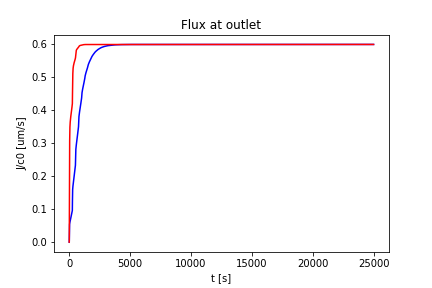
\includegraphics[width=\linewidth]{figs/flux}
	\label{fig:flux}
\end{figure}

\begin{figure}[h]
	\centering
	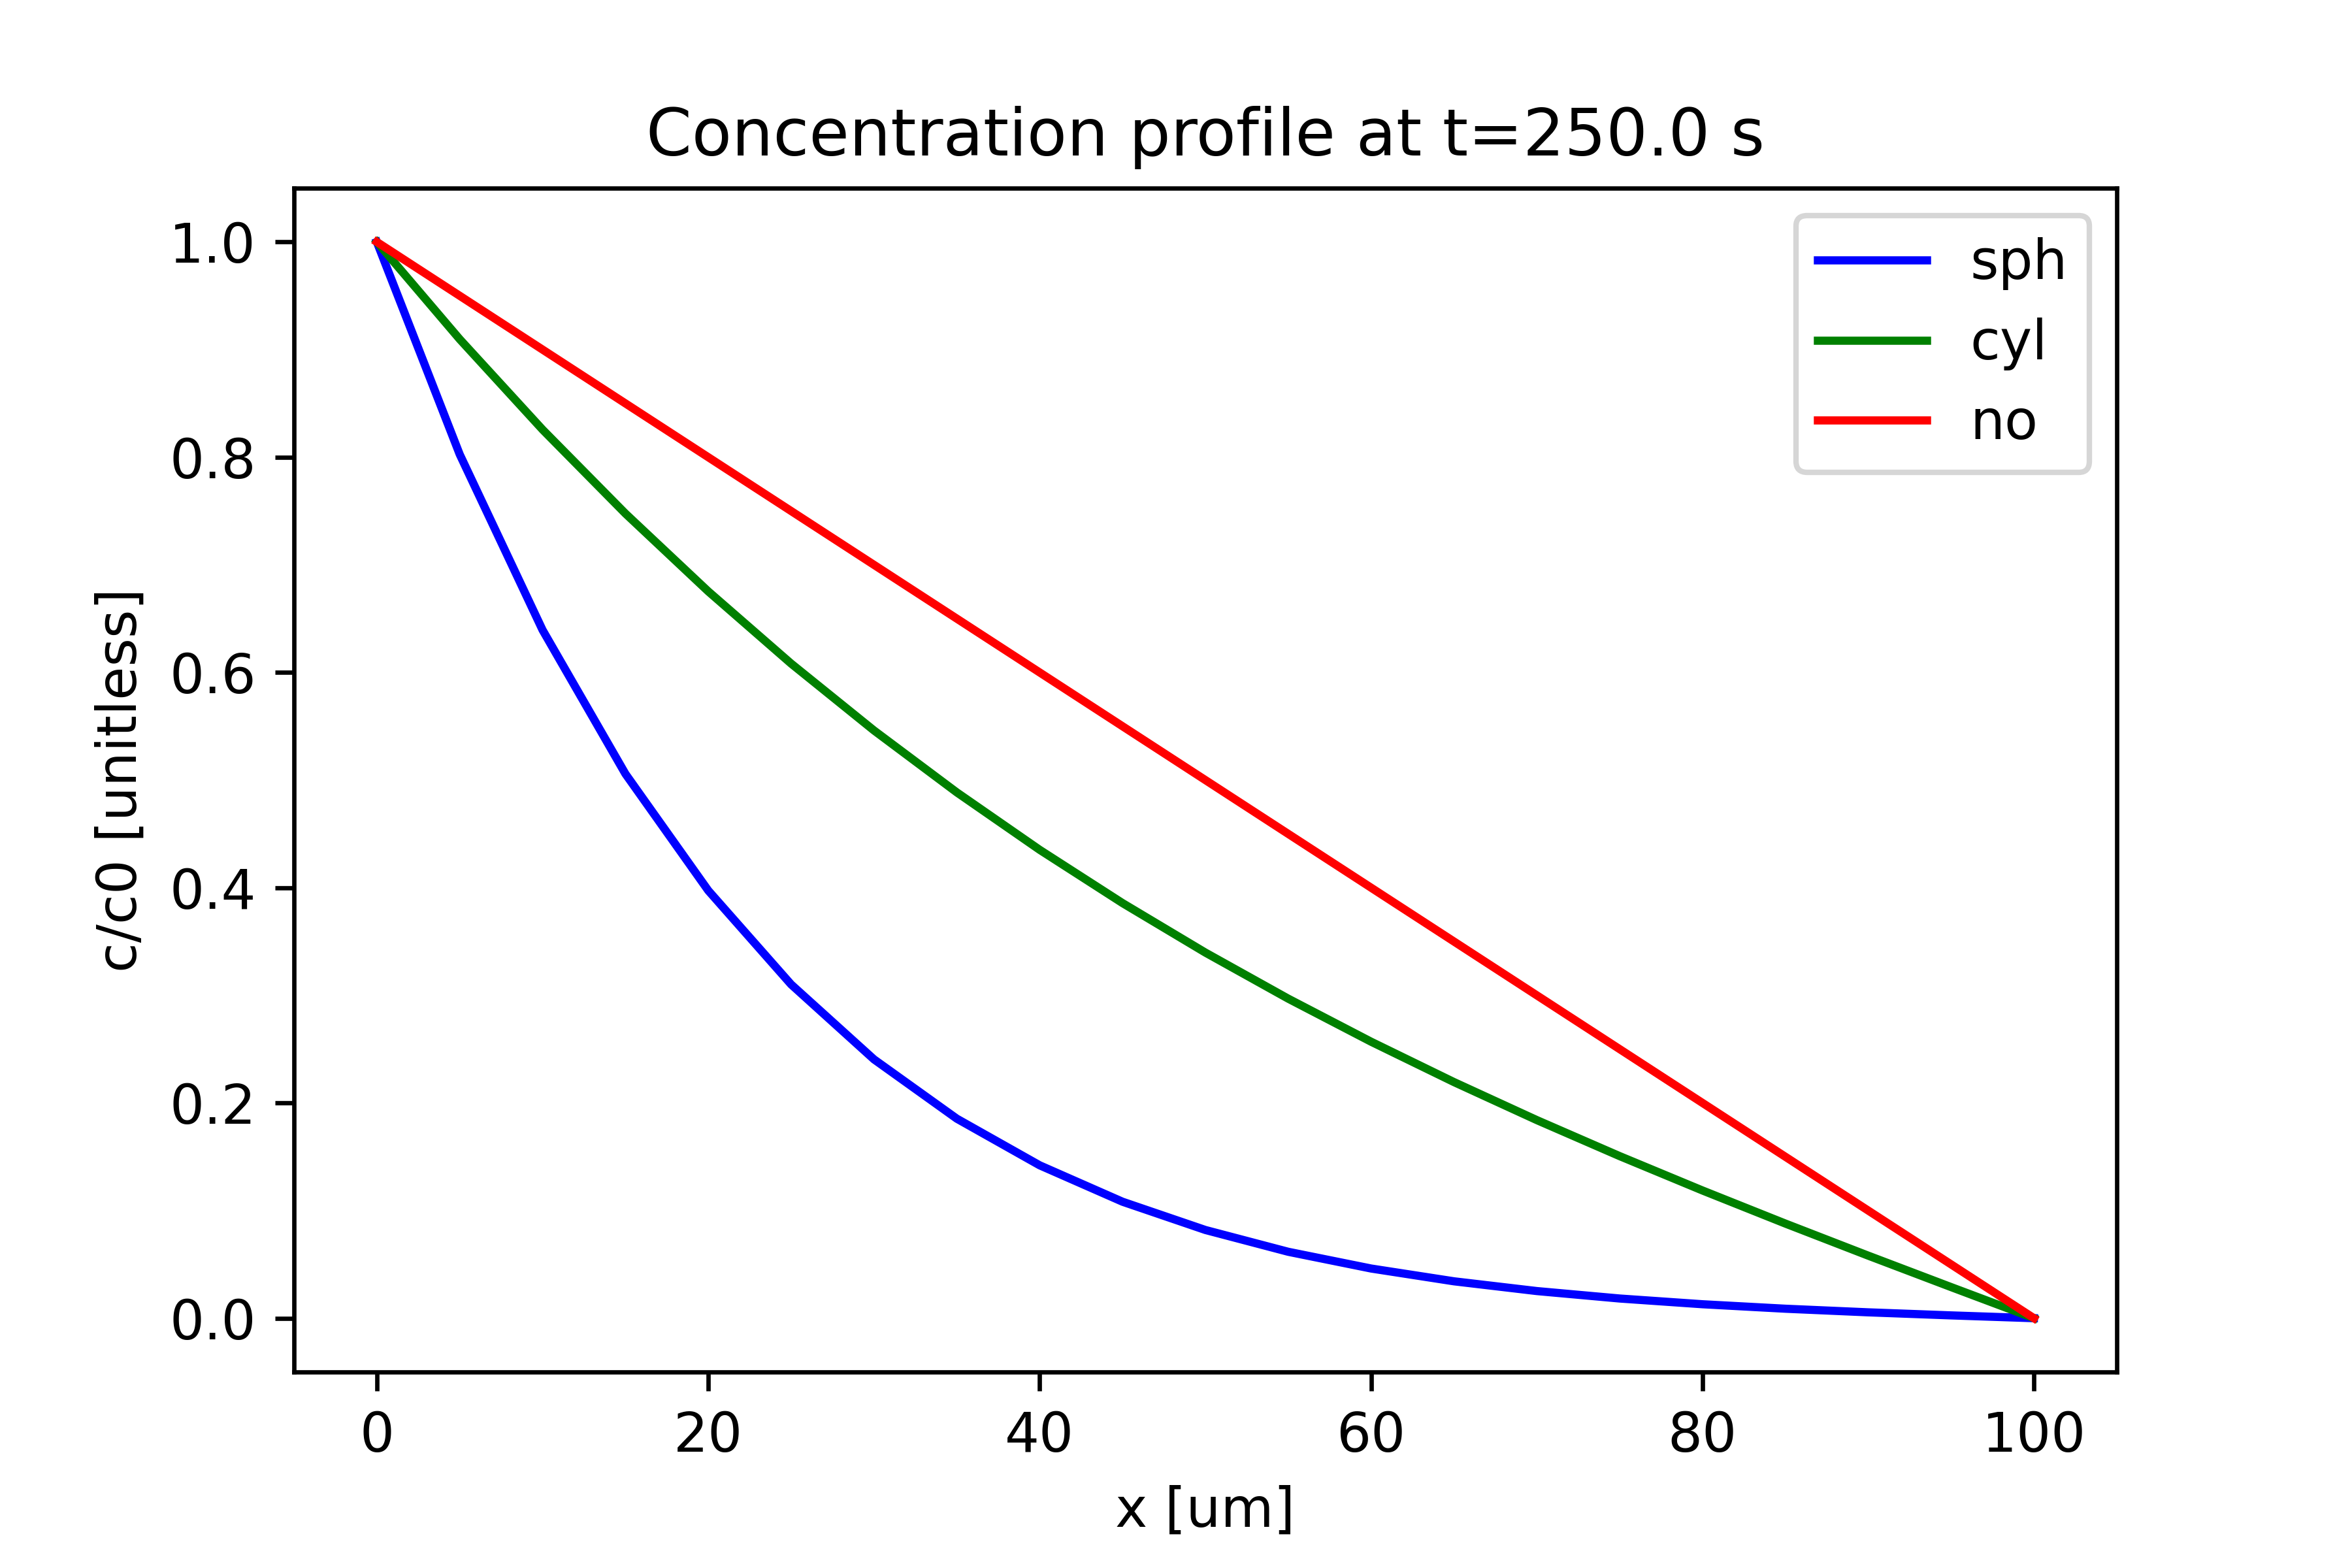
\includegraphics[width=\linewidth]{figs/profile999}
	\label{fig:profile999}
\end{figure}

\begin{figure}[h]
	\centering
	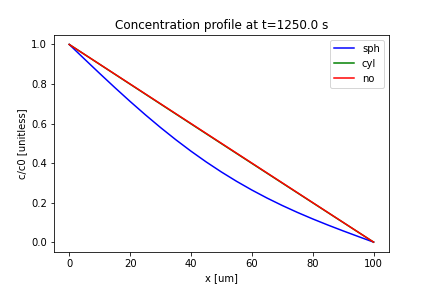
\includegraphics[width=\linewidth]{figs/profile4999}
	\label{fig:profile4999}
\end{figure}

\appendix
\section{Transform approaches}
\subsection{Fourier transforming bulk equation}
We can do other things. Let's try to Fourier transform this (in $t$). Let $C(x,s) = \mathcal{F}_t(c(x,t))(s)$. Hence, we have that
\begin{equation}
\mathcal{F}_t\left(\pderiv{}{t}c(x,t) \right)(s) = 2 \pi i s C(x,s)
\end{equation}
\begin{equation}
\mathcal{F}_t\left(\sum_{k=1}^\infty (\omega_k *_t c')(x,t)\right) = C(x,s) \sum_{k=1}^\infty \frac{1}{1 - i\frac{\alpha \pi^2 k^2}{2 R^2 \pi s}},
\end{equation}
or
\begin{equation}
\mathcal{F}_t\left(\sum_{k=1}^\infty (\omega_k *_t c')(x,t)\right) = C(x,s) \sum_{k=1}^\infty \frac{1}{1 + \left(\frac{\alpha \pi^2 k^2}{2 R^2 \pi s}\right)^2}\left(1 + i\frac{\alpha \pi^2 k^2}{2 R^2 \pi s}\right),
\end{equation}
and the diffusive term stays the same. Hence, joining everything
\begin{equation}
C(x,s) \zeta(s) = D \frac{\partial^2 C}{\partial x^2}(x,s),
\end{equation}
with
\begin{equation}
\zeta(s) = 2 \pi i s + 8 \pi R \Gamma \alpha K \sum_{k=1}^\infty \frac{1}{1 - i \frac{A k^2}{s}}; \quad A = \frac{\alpha \pi}{2 R^2}
\end{equation}

\subsection{Laplace transforming bulk equation}
In a similar manner, we try Laplace transform then. Let $\mathcal{C}(x,s) = \mathcal{L}_t(c(x,t))(s)$. 
He have that
\begin{equation}
\mathcal{L}_t\left(\pderiv{}{t}c(x,t) \right)(s) = s \mathcal{C}(x,s) - c(x,0),
\end{equation}
and
\begin{equation}
\mathcal{L}_t\left(\sum_{k=1}^\infty (\omega_k *_t c')(x,t)\right) = (s \mathcal{C}(x,s) - c(x,0)) \sum_{k=1}^\infty \frac{1}{1 + \frac{\alpha \pi^2 k^2}{R^2} s}
\end{equation}
\begin{equation}
\sum_{k=1}^\infty \frac{1}{1 + \frac{\alpha \pi^2 k^2}{R^2} s} = \frac{1}{2}\left(\sqrt{\frac{R}{\alpha}} s^{-1/2} \coth \left(\sqrt{\frac{R}{\alpha}} s^{-1/2}\right) - 1 \right).
\end{equation}
Since we assumed $c(x,0) = 0$, the equation for $\mathcal{C}$ becomes
\begin{equation}
\begin{split}
& \mathcal{C}(x,s) \xi(s) = \frac{\partial^2 \mathcal{C}}{\partial x^2}(x,s) \\
& \xi(s) = \frac{s}{D} \left(1 + \frac{\beta}{2} \left(\sqrt{\frac{R}{\alpha s}} \coth \left(\sqrt{\frac{R}{\alpha s}} \right) - 1 \right) \right)
\end{split}.
\end{equation}

We must have
\begin{equation}
\mathcal{C}(x,s) = A(s) e^{\sqrt{\xi(s)} x} + B(s) e^{-\sqrt{\xi(s)} x}
\end{equation}

Using Dirichlet conditions $c(0,s) = c_0$, $c(L,s) = 0$, we have that $\mathcal{C}(0,s) = c_0/s$, $\mathcal{C}(L,0) = 0$, and we find $A(s), B(s)$ solving the system
\begin{equation}
\begin{bmatrix}
1 & 1 \\
e^{\sqrt{\xi(s)} L} & e^{-\sqrt{\xi(s)} L}
\end{bmatrix} \begin{bmatrix} A(s) \\ B(s) \end{bmatrix} = \begin{bmatrix} c_0/s \\ 0 \end{bmatrix},
\end{equation}
We have that
\begin{equation}
\begin{split}
& A(s) = \frac{e^{-\sqrt{\xi(s)} L}}{e^{-\sqrt{\xi(s)} L} - e^{\sqrt{\xi(s)} L}} \frac{c_0}{s} \\
& B(s) = -\frac{e^{\sqrt{\xi(s)} L}}{e^{-\sqrt{\xi(s)} L} - e^{\sqrt{\xi(s)} L}} \frac{c_0}{s}
\end{split}
\end{equation}
Then, we have that
\begin{equation}
\mathcal{C}(x,s) = \frac{c_0}{s \left(e^{-\sqrt{\xi(s)} L} - e^{\sqrt{\xi(s)} L}\right)} \left(e^{-\sqrt{\xi(s)}(L-x)} - e^{\sqrt{\xi(s)}(L-x)}\right)
\end{equation}
Or, simplifying
\begin{equation}
\frac{c_0}{s} \frac{\sinh(\sqrt{\xi(s)}(L-x))}{\sinh(\sqrt{\xi(s)} L)}
\end{equation}
For each $x$, Laplace-invert $\mathcal{C}(x,s)$. Have no idea how tough this is numerically.

\end{document}
